\question{Теорема Шокли-Рамо}

Соотношение (\ref{eq24.1.18}) для областей 1 и 3 можно преобразовать следующим 
образом:
\begin{equation}
	i_\text{пов} = |q|v\frac{E}{U}
	\label{eq25.1.24}
\end{equation}

Здесь величина \( E = U/d \), а отношение \( E/U \) можно рассматривать как 
коэффициент, соответствующий некоторому распределению напряженности поля в 
пространстве при подаче на анод единичного потенциала при отсутствии в диодном 
промежутке заряженных частиц. В общем случае, когда направление движения 
электронов и направление вектора электрической индукции не совпадают, 
(\ref{eq25.1.24}) следует переписать в виде
\[
	i_\text{нав} = -|q|\left( \frac{\vec{E}\cdot\vec{E}}{U} \right)
\]

Это соотношение, а точнее, его интегральное представление, когда всё 
пространство между электродами заполнено движущимися зарядами, представляет 
теорему Шокли-Рамо:
\[
	i_\text{нав} = -\int |dq|\left( \frac{\vec{E}\cdot\vec{E}}{U} \right) = 
		-\int\limits_V |\rho| \frac{(\vec{E}\cdot\vec{E})}{U} dV = 
		-\int\limits_V \left( \frac{\vec{j}_k\cdot\vec{E}}{U} \right)dV
\]
Она гласит: \emph{величина тока, наведенного на электроде, определяется как 
интеграл по всему объёму, занятому частицами, от скалярного произведения 
конвекционного тока на напряженность электрического поля при условии подачи 
на заданные электрод единичного потенциала и соединении и закорачивании на 
землю всех остальных электродов.}

При этом следует учесть, что величина \( E/U \) является нормированной 
величиной напряженности поля в точке, где находится заряд, при отсутствии 
любых зарядов в пространстве.

Докажем эту теорему достаточно строго для отдельного электрона, двигающегося 
в некотором пространстве, окруженном проводящими электродами 
(\ref{img25.1.3}). В этом случае её можно представить в виде
\[
	i = E_v qv
\]

\begin{figure}[h!]
	\center
	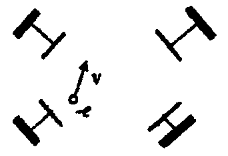
\includegraphics[width=.4\textwidth]{25_1} \hspace{1em}
	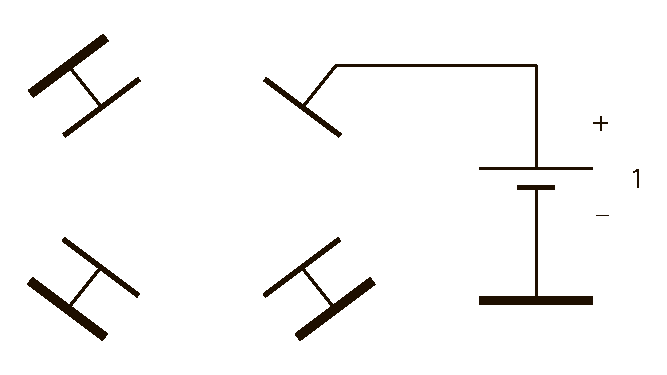
\includegraphics[width=.4\textwidth]{25_2}
	\parbox{.4\textwidth}{\caption{Электрон в пространстве, окруженном 
		системой проводящих заземленных электродов}
	\label{img25.1.3}} \hspace{1em}
	\parbox{.4\textwidth}{\caption{Изображение пространства, окруженного 
		проводящими электродами}
    \label{img25.1.4}}
\end{figure}

Здесь: \( v \) -- скорость движения заряда, \( E_v \) -- взята вдоль 
направления движения электрона составляющая электрического поля, которое 
существовало бы в точке нахождения заряда при его отсутствии, когда 
потенциал того электрода, на котором определяется наведенный ток, на единицу 
выше потенциала остальных электродов, которые, в свою очередь, заземлены.

Сначала рассмотрим состояние, когда все электроды заземлены, а между ними 
движется со скоростью \( v \) электрон \( -e \). В этом случае потенциал, 
создаваемый зарядом, является функций координат и времени
\[
	\phi = \phi( x, y, z, t )
\]

Если окружить заряд сферой с очень малым радиусом, можно считать, что 
потенциал на его поверхности постоянен и равен \( \phi_q \). Используя 
теорему Гаусса для поверхности сферы, окружающей заряд, можно записать 
следующее соотношение:
\[
	\int\limits_S (\vec{E}\vec{n}) dS = -\frac{e}{\eps_0}
\]
где \( \vec{E} \) -- вектор напряженности электрического поля; 
\( \vec{n} \) -- нормаль к поверхности \( S \).

Для второго состояние системы, когда поле создаётся одним электродом, на 
который подаётся единичный потенциал (\ref{img25.1.4}), потенциал в 
пространстве является функцией только координат 
\( \phi' = \phi'( x, y, z ) \). Тогда в точке, где должен находится электрон, 
этот потенциал \( \phi'_q = \phi'( x_q, y_q, z_q ) \). Следует помнить, что  
для первого случая решение уравнения Лапласа \( \Delta\phi = 0 \) справедливо 
для всех точек пространства, исключая область сферы с зарядом и поверхности 
электродов, а для второго случая -- везде, кроме объёма электродов. Если 
теперь воспользоваться преобразованием Грина
\begin{equation}
	\int\limits_S (\phi' grad_n\phi - \phi grad_n\phi') dS = 
		\int\limits_V (\phi'\Delta\phi - \phi\Delta\phi') dV
	\label{eq25.1.28}
\end{equation}
где \(  grad_n\phi = \pder{\phi}{n} \) и 
\(  grad_n\phi' = \pder{\phi'}{n} \) -- производные \( \phi \) и \( \phi' \) 
по внешней нормали к элементу поверхности \( dS \) ограничивающей объём 
\( V \); \( \phi \) и \( \phi' \) -- непрерывные, дважды дифференцируемые 
функции координат. Поскольку для всего объёма пространства, исключая объём 
сферы, выполняется уравнение Лапласа, то объёмный интеграл
\[
	\int\limits_V (\phi'\Delta\phi - \phi\Delta\phi') dV = 0
\]
и уравнение (\ref{eq25.1.28}) принимает вид
\begin{equation}
	\int\limits_S \left(
		\phi'\pder{\phi}{n} - \phi\pder{\phi'}{n}
	\right) dS = 0
	\label{eq26.1.29}
\end{equation}

Исходя из условий задачи данный интеграл можно разбить на три части:
\begin{enumerate}\itemsep-2pt
	\item интеграл по поверхности электродов, которые заземлены в обеих 
		системах (рис.\ref{img25.1.3} и рис.\ref{img25.1.4}); это 
		поверхность -- \( S_{n-1} \);
	\item интеграл по поверхности того электрода, на который подан единичный 
		потенциал; это поверхность -- \( S_1 \);
	\item интеграл по поверхности малой сферы, окружающей электрон; это 
		поверхность -- \( S_q \)
\end{enumerate}

Первый интеграл тождественно равен нулю из-за того, что все потенциалы 
заземленных электродов равны нулю. Второй интеграл
\[
	\int\limits_{S_1} \left(
		\phi'\pder{\phi}{n} - \phi\pder{\phi'}{n}
	\right) dS = \phi'\int\limits_{S_1} \pder{\phi}{n} dS = 
		\int\limits_{S_1} \pder{\phi}{n} dS
\]

Для определения третьего интеграла воспользуемся условием постоянства 
потенциала на поверхности \( S_q \), в связи с чем получаем
\[
	\int\limits_{S_q} \left(
		\phi'_q\pder{\phi}{n} - \phi_q\pder{\phi'}{n}
	\right) dS = \phi'_q\int\limits_{S_q} \pder{\phi}{n} dS -
		\phi_q\int\limits_{S_q} \pder{\phi'}{n} dS
\]

Поскольку \( \phi'_q \) представляет потенциал для случая отсутствия электрона 
внутри малой сферы, то \( \int\limits_{S_q} \pder{\phi'}{n} dS = 0 \), и 
уравнение (\ref{eq25.1.29}) приводится к следующему виду:
\[
	\phi'_q\int\limits_{S_q} \pder{\phi}{n} dS + 
		\int\limits_{S_1} \pder{\phi}{d} dS = 0
\]

Воспользуемся теоремой Гаусса и введём заряды:
\[
	\int\limits_{S_1} \pder{\phi}{d} dS = \frac{q_1}{\eps_0};\quad
	\int\limits_{S_q} \pder{\phi}{n} dS = -\frac{e}{\eps_0} \text{ или }
	q_1 - e\phi'_q = 0 
\]

По определению, наведенный ток в цепи электрода с единичным потенциалом
\[
	i_1 = i_n = \frac{dq_1}{dt} = e\frac{d\phi'_q}{dt}
\]
Если при этом выбрать координату \( z \) в направлении движения электрона, то 
\[
	i_n = e\frac{d\phi'_q}{dt} = e\frac{d\phi'_q}{dz}\frac{dz}{dt}
\]
В результате, поскольку \( d\phi'_q/dz = -E_z = -E_v \) и \( dz/dt = v \), 
получаем выражение для наведенного тока 
\begin{equation} 
	i_n = -E_v ev
	\label{eq25.1.31}
\end{equation}
совпадающее с (\ref{eq25.1.28}).

При наличии распределенной системы зарядов уравнение (\ref{eq25.1.31}) следует 
представить в интегральной форме
\[
	i_\text{н} = -\int\limits_V \rho(\vec{E}\vec{v}) dV
\]